\section{Laboratorium nr 1}

\subsection{Wprowadzenie do programu Matlab/GNU Octave}

Zarówno MATLAB jak i~GNU Octave są programami przeznaczonymi do numerycznych obliczeń macierzowych. Posiadają wiele funkcji bibliotecznych i~narzędzi wizualizacyjnych, które sprawiają, że owe programy idealnie się sprawdzają w zastosowaniach takich jak: statystyka, przetwarzanie sygnałów, teoria sterowania, czy uczenie maszynowe i~big data. Programy te posiada rozbudowane funkcje i~wiele toolbox'ów, które sprawiają, że są przydatne w dużej liczbie dziedzin inżynieryjnych, ekonomicznych czy statystycznych. Wszystkie poznane na tych zajęciach zagadnienia powinny być również łatwe do implementacji w innych programach np. w Pythonie.

Podczas pierwszych zajęć laboratoryjnych studenci powinni zaznajomić się, z~podstawowymi poleceniami, funkcjami programu MATLAB/Octave. Jest to niezbędne, do późniejszego zgłębiania zagadnień związanych z~cyfrowym przetwarzaniem sygnałów.


\subsubsection{Podstawowe polecenia i funkcje}
Pierwotnie MATLAB, był głównie używany do wykonywania operacji macierzowych. Aby utworzyć nową macierz i~przypisać ja do zmiennej należy wpisać w oknie \texttt{Command Windows} polecenie:
\begin{lstlisting}[caption=Tworzenie macierzy będącej kwadratem magicznym, label=lab1/lst/magicMatrix]
>> A = [16 3 2 13; 5 10 11 8; 9 6 7 12; 4 15 14 1]
\end{lstlisting}
Średnikiem oddzielane są poszczególne wiersze macierzy. Po wpisaniu powyższej macierzy dalej mamy możliwość wykorzystywanie tej zmiennej, jest ona zachowana w przestrzeni roboczej programu MATLAB/Octave. Jeśli wyrażeniu nie przypiszemy wartości do konkretnej liczby to program przypisze ją do zmiennej \texttt{ans}, aby zachować wynik danego wyrażenia. 

Na tak stworzonej macierzy można wykonywać operacje sumowania, transpozycji czy wyznaczenia wartości znajdujących się na przekątnej, odwracania macierzy i~obliczania wyznacznika.
\begin{lstlisting}[caption=Przykładowe funkcje przydatne podczas pracy z macierzami , label=lab1/lst/matrixFunctions]
>> sum(A) % sumowanie wartosci z kolejnych kolumn
>> A' % transpozycja macierzy
>> diag(A) % wartosci znajdujace sie na przekatnej
>> inv(A) % odwracanie macierzy
>> det(A) % oblicza wyznacznik z macierzy
\end{lstlisting}

Często konieczne jest odwołanie się do konkretnego zakresu elementów macierzy, bądź pojedynczej wartości. Pobieranie tych danych zrealizowane jest przez podanie odpowiednich zakresów w nawiasach przy nazwie utworzonej macierzy. \textbf{W programach MATLAB/GNU Octave indeksy tablic są numerowane liczby jeden!}
\begin{lstlisting}[caption=Odwoływanie się do elementów macierzy , label=lab1/lst/matrixElements]
>> A(1,2) % wypisuje wartosc elementu znajdujacego sie w pierwszym wierszu i drugiej kolumnie
>> A(:,2) % wypisuje wartosci elementow znajdujacych sie w drugiej kolumnie
>> A(1:3,2) % wypisuje wartosci elementow znajdujacych sie w drugiej kolumnie i pierwszych trzech wierszach
\end{lstlisting}

W wielu sytuacjach konieczne okazuje się tworzenie wektora z~użyciem operatora dwukropka, albo przy użyciu funkcji \texttt{zeros}, \texttt{ones} czy \texttt{linspace}. 
\begin{lstlisting}[caption=Tworzenie macierzy z wykorzystaniem funkcji oraz operatora \texttt{:} , label=lab1/lst/matrixZerosOnesLinespace]
>> B = 1:10 % tworzy wektor B skladajcy sie z wartosci od jeden do dziesiec inkrementowanych z krokiem jeden
>> B = 1:0.1:10 % tworzy wektor jak wyzej jednak krok w tym przypadku wynosi 0.1
>> B = 2.^[1:4] % tworzy wektor ciagu geometrycznego o ilorazie 2
>> B = zeros(2,4) % tworzy wektor 2x4 skladajacy sie z samych zer
>> B = ones(3,4) % tworzy wektor 3x4 skladajacy sie z samych jedynek
>> B = linspace(3,42) % tworzy wektor 100 elementow ronomiernie rozlozonych pmiedzy wartosciami 3 i 42
>> B = linspace(3,42,50) % tworzy wektor 50 elementow roznomiernie rozlozonych pomierzy wartosciami 3 i 42
\end{lstlisting}

Na macierzach w programie MATLAB/Octave możliwe jest wykonywanie operacji arytmetycznych zgodnie z~zasadami wykonywania działań na macierzach.
\begin{lstlisting}[caption=Operacje arytmetyczne na macierzach , label=lab1/lst/matrixOperations]
>> C = [1 2 3]+[1 2 3]
>> C = [1 2 3]*[4; 5; 6]
>> C = [1 2 3]'*[4 5 6]
>> C = [1 2 3]^2 % [1 2 3]*[1 2 3]
>> C = [1 2 3].^2 % operator ^ zapisany z poprzedzajaca go kropka powoduje wykonywanie operacji potegowania osobno dla kazdego elemetu
>> C = [1 2 3].*[1 2 3] % wykonuje operacje mnozenia element po elemencie
\end{lstlisting}

W omawianych programach można korzystać z~wielu gotowych stałych i~funkcji. 
\begin{lstlisting}[caption=Przykładowe stałe i funkcje , label=lab1/lst/constantsAndFucntions]
>> pi % 3.141592...
>> i~% reprezentuje wartosc urojona
>> j % jak wyzej
>> [2 + 2i]*[3 + 3i] % (6 + 6i + 6i + 6i^2) = (0 + 12i)
>> Inf % nieskoczonosc
>> NaN % not a number
>> sqrt(256) % oblicza pierwiastek
>> abs(-12) % obliczna wartosc bezwglednia
>> exp(7) % eksponent z liczby siedem e^7
>> sin(pi/2) % wartosc pi dla argumetu pi/2
>> log10(100) % operacje obliczania logarytmu dziesietnego
>> mean([1 2 3 4 5 6]) % oblicza wartosc oczekiwana z wektora liczb
>> var([4 5 6 5 4 6]) % oblicza wariancje z wektora liczb
>> min([1 2 3 5 -50])
>> max([1 2 3 5 -50])
\end{lstlisting}

Aby dodać do macierzy albo z~niej usunąć konkretną kolumnę bądź wiersz można posłużyć się operatorem \texttt{[]}:
\begin{lstlisting}[caption=Usuwanie i dodawanie wierszy/kolumn do macierzy , label=lab1/lst/matrixAddRemoveRowColumn]
>> X = [1 2 3; 4 5 6; 7 8 9]
>> X(:,2) = [] % usuwa druga kolumne z macierzy
>> X = [X; [10 11 12]] % dodaje wiersz do macierzy
\end{lstlisting}

Funkcja \texttt{find} pozwala na znalezienie elementów macierzy, które spełniają wyrażenie logiczne. \texttt{find} zwraca indeksy pod którymi przechowywane są te elementy.
\begin{lstlisting}[caption=Szukanie elementów macierzy spełniających warunek logiczny , label=lab1/lst/findFunction]
>> X = [1 2 3; 4 NaN 6; 7 8 NaN]
>> find(isnan(X))
>> find(X>3)
\end{lstlisting}

\subsubsection{Tworzenie skryptów i~funkcji}
Zamiast wpisywać kolejne komendy w wierszu poleceń, MATLAB/Octave umożliwia tworzenie tzw. m-plików, które są skryptami zawierającymi szereg kolejno wykonujących się poleceń czy wywołań funkcji. Jeśli chcemy uruchomić skrypt z~poziomu wiersza poleceń wystarczy napisać jego nazwę i~zatwierdzić enterem (jeśli aktualnie nad danym skryptem pracujemy, jest on uruchomiony w oknie programu \texttt{Editor}, można również go uruchomić za pomocą przycisku F5). 

Analogicznie MATLAB/Octave pozwala na pisanie własnych funkcji, które później mogą być wywoływane z~określonymi argumentami i~mogą zwracać jedną bądź wiele wartości. Definicja funkcji wygląda w~następujący sposób:
\begin{lstlisting}[caption=Prototyp funkcji w programie MATLAB/Octave , label=lab1/lst/matlabFunctionPrototype]
	function [y1,...,yN] = myfun(x1,...,xM)
\end{lstlisting} 
Ze względu na tzw. duck typing, nie ma konieczności deklarowania typu przekazywanej/zwracanej wartości.


\subsubsection{Rysowanie wykresów}
MATLAB/Octave posiada bogate możliwości wizualizacji danych, z~których podczas zajęć laboratoryjnych będziemy korzystać regularnie. Podstawową funkcją, która odpowiada za rysowanie wykresów jest \texttt{plot}. Pierwszym argumentem przekazywanym do tej funkcji jest wektor zawierający liczby znajdujące się osi X, natomiast drugim jest wektor zawierający odpowiadające im wartości (oś Y).
\begin{lstlisting}[caption=Rysowanie funkcji $sin$ na jednym wykresie, label=lab1/lst/plotSin]
x = 0:pi/100:2*pi; % tworzenie wektora czasu
y1 = sin(x); % oblicza wartosci funkcji sin dla wektora czasu x
y2 = sin(x-0.25);
y3 = sin(x-0.5);

figure % tworzy nowy uchwyt na wykres
plot(x,y1,x,y2,'--',x,y3,':') % narysuj na jednym wykresie trzy przebiegi funkcji sinus

figure % utworz nowy uchyt na wykres
plot(x, y1) % narysuj pierwsza funkcje y1
hold on % zachowaj wczesniej narysowany wykres
plot(x, y2) % narysuj wykres y2 obok wczenisjeszgeo y1
plot(x, y3) % dodaj trzeci wykres y3
\end{lstlisting}

Czasami może okazać się konieczne podzielenie jednego rysunku na kilka mniejszych rozmieszczonych w określonej kolejności. Pomocna w takim przypadku okazuje się funkcja \texttt{subplot}:
\begin{lstlisting}[caption=Rysowanie funkcji $sin$ na współdzielonym wykresie , label=lab1/lst/subplotSin]
subplot(2,2,1) % narysowany ponizsza funkcja plot wykres znajdzie sie na pierwszych miejscu na podzielonym na cztery obszary (2x2) rysunku 
x = linspace(0,10);
y1 = sin(x);
plot(x,y1)
title('Subplot 1: sin(x)')

subplot(2,2,2) % narysowany ponizsza funkcja plot wykres znajdzie sie na drugim miejscu na podzielonym na cztery obszary (2x2) rysunku 
y2 = sin(2*x);
plot(x,y2)
title('Subplot 2: sin(2x)')

subplot(2,2,3)
y3 = sin(4*x);
plot(x,y3,'ks')
title('Subplot 3: sin(4x)')

subplot(2,2,4)
y4 = sin(8*x);
plot(x,y4, 'r:+)
title('Subplot 4: sin(8x)')
\end{lstlisting}

Na powyższym przykładzie przy rysowaniu niektórych wykresów wykorzystano markery zmieniające styl i~kolory rysowanych przebiegów:
\begin{itemize}
	\item zdefiniowane kolory: \texttt{'c','m','y','r','g','b','w','k'} odpowiadają one kolejno kolorom: niebieskozielonym, różowym, żółtym, czerwonym, zielonym, niebieskim, białym i~czarnym;
	\item style linii: \texttt{-} ciągła linia, \texttt{-}\texttt{-} linia przerywana, \texttt{:} linia wykropkowana, \texttt{-.} linia przerywana myślnikiem i~kropką;
	\item typy markerów: \texttt{+},\texttt{o}, \texttt{*}, \texttt{x}, \texttt{s} (kwadrat), \texttt{d} (romb), \texttt{\^{},>,v,<} (trójkąty zwrócone w różne strony), \texttt{p} (pentagram) i~\texttt{h} (heksagram). 
\end{itemize}

Jeśli konieczne jest ustalenie zakresów osi XY należy użyć funkcji \texttt{axis([xmin xmax ymin ymax])}, jeśli sami nie ustalimy tych zakresów MATLAB/Octave ustali je automatycznie. Włączenie widocznej siatki na wykresie można zrealizować za pomocą wyrażenia: \texttt{grid on}. Opisy poszczególnych osi tworzy się za pomocą funkcji: \texttt{xlabel} i~\texttt{ylabel} natomiast legendę do wykresów za pomocą \texttt{legend}. Do ustawienia tytułu wykresu korzystamy natomiast z~wyrażenia: \texttt{title}.
\begin{lstlisting}[caption=Nazywanie osi dodawanie tytułu oraz legendy i zmiana zakresów osi układu współrzędnych , label=lab1/lst/plotLabelsTitleAxisLegend]
t = -2*pi:pi/100:2*pi;
y1 = sin(t);
y2 = cos(t);
plot(t,y1);
hold on
plot(t, y2);
axis([-2*pi 2*pi -1 1]);
xlabel('-2\pi \leg {\itt} \leg 2*\pi')
ylabel('f(x)')
title('My plot');
legend('sin(x)','cos(t)');
\end{lstlisting} 

\subsubsection{Instrukcje warunkowe/pętle}
MATLAB/Octave posiada wiele konstrukcji pozwalających na sterownie przepływem programu. Tak jak w większości znanych języków w MATLAB/Octave można korzystać z~instrukcji warunkowych \texttt{if-else}, pętli \texttt{for}, \texttt{while} czy \texttt{switch-case}. 

Przykładowe użycie instrukcji warunkowej \texttt{if-else} zostało pokazane na poniższym listingu~\ref{lab1/lst/ifElse}. Fragment programu wykonuje porównanie dwóch liczb i~wypisuje na ekranie konsoli informację o~wyniku tego porównania. Dalej zostało pokazane użycie pętli \texttt{for}~\ref{lab1/lst/forLoop}. Widać, że pętla zachowuje się jak \texttt{foreach}, iteruje ona wektor znajdujący się po prawej stronie znaku \texttt{=}. 
\begin{lstlisting}[caption=Porównywanie dwóch liczb z wykorzystaniem instrukcji \texttt{if-else}, label=lab1/lst/ifElse]
A = 12;
B = 14
if A > B
	disp('Greater')
elseif A < B
	disp('Less')
elseif A == B
	disp('Equal')
else
	disp('Can not be evaluated')
end
\end{lstlisting} 

\begin{lstlisting}[caption=Trzy pętle \texttt{for} wykonujące się na różnych przedziałach wektora \texttt{i}, label=lab1/lst/forLoop]
for i = 1:10
	disp(i)
end

for i = 1.0:-0.2:0.0
	disp(i)
end

for i = [1 4 5 10 -8]
	disp(i)
end
\end{lstlisting} 

Na tych zajęciach nie będziemy poruszać możliwości programowania obiektowego w języku MATLAB/Octave, tym niemniej należy wspomnieć, że w~omawianych językach możliwe jest tworzenie własnych typów (klas). Przy bardziej złożonych problemach, szczególnie przy operowaniu na dużej ilości danych, wykorzystanie obiektów pozwala znaczenie uprościć wykonywaną pracę.





\subsection{Szumy}\label{lab1/sec/noises}

W cyfrowym przetwarzaniu sygnałów często będziemy mieć do czynienia z szumami, które w~przeciwieństwie do sygnałów deterministycznych nie są opisane przez żadne znane zależności matematyczne. Szum jest procesem losowym, jednak posiada pewne cechy, które go definiują. Jeśli rozważymy np. rzuty kostką, to rozkład gęstości prawdopodobieństwa takiej zmiennej losowej będzie przyjmował kształt ,,prostokąta'' (rozkład równomierny). Prawdopodobieństwo wylosowania konkretnej liczby oczek wynosi $\frac{1}{6}$. Wiele rzeczywistych procesów losowych posiada jednak gaussowski rozkład gęstości prawdopodobieństwa np. szumy termiczne czy promieniowanie. W~przetwarzaniu obrazów szumy gaussowskie mogą być powodowane przez niewystarczające naświetlenie, wysoką temperaturę czy szum elektryczny. Z szumem gaussowskim bardzo często możemy się spotkać w~rzeczywistych procesach. Np. w kontekście szumu termicznego, zaburzenia są powodowane ogromną liczbą losowo oscylujących cząsteczek, pobudzanych przez energię cieplną.

\begin{figure}[hbt!]
	\centering
	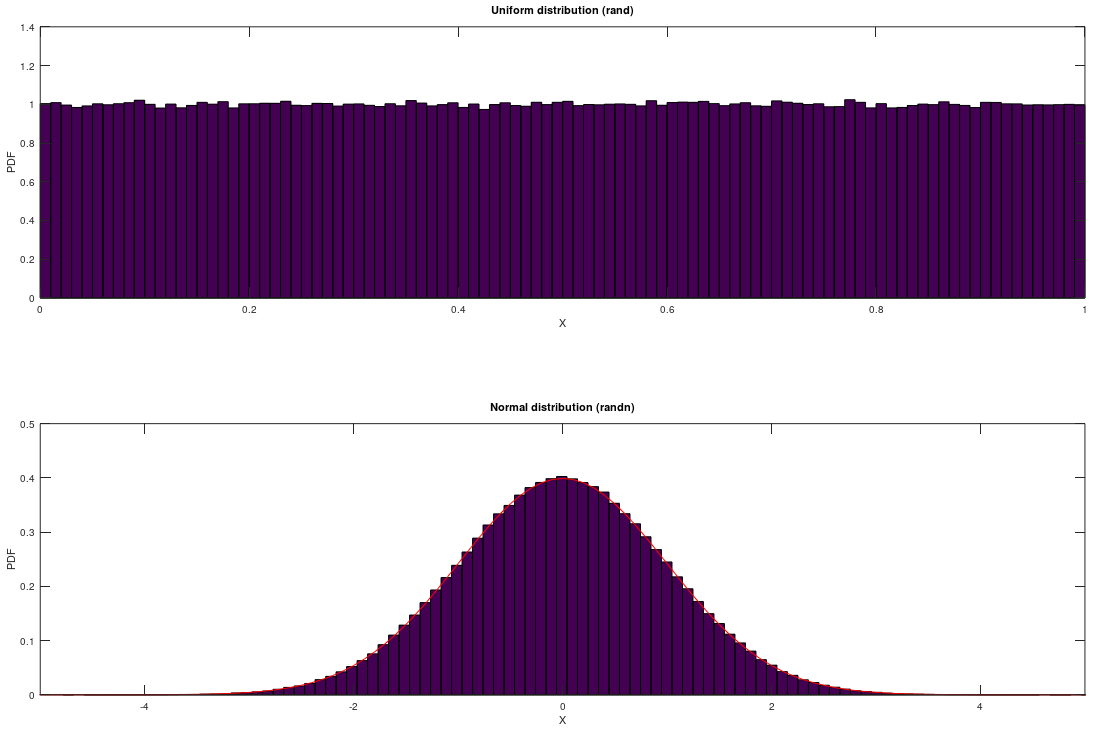
\includegraphics[width=0.9\linewidth]{images/whiteNoisePdf}
	\caption{Wykresy gęstości prawdopodobieństwa dla szumu o rozkładzie równomiernym oraz normalnym.}
	\label{lab1/fig/whiteNoisesPdf}
\end{figure}


Oba wymienione powyżej szumy są szumami białymi. Oznacza to, że składają się one z~mieszaniny różnych częstotliwości, które powodują, że takie szumy posiadają płaskie widmo~\footnote{Obraz uzyskany w~wyniku rozłożenia danego sygnału na szereg składowych o różnych częstotliwościach występujących w~tym sygnale}.
%W akustyce częsciej korzysta się szumu różowego, które posiada widmo opadające o 3dB na oktawę (10dB na dekadę). Spowodowane jest to tym, jak ludzie ucho odbiera bodzće dźwiękowe (logarytmicznie, a nie liniowo).


Rozkład równomierny:
\begin{equation}\label{lab1/eq/uniformDistribution}
	p(x_0) =
	\begin{cases} 
		\frac{1}{b-a} & \text{dla $a  \leq  x_0  \leq  b$} \\
		0 & \text{dla pozosotałych $x_0$}
	\end{cases}
\end{equation}

Rozkład normalny:
\begin{equation}\label{lab1/eq/normalDistribution}
	p(x_0) = \frac{1}{\sqrt{2\pi\sigma^2}} exp\left[-\frac{(x_0 - \bar{x}^2)}{2\sigma^2} \right]
\end{equation}

W MATLABie/Octavie do utworzenia wektora zawierającego próbki szumu, można wykorzystać funkcję \texttt{rand} dla rozkładu równomiernego, \texttt{randn} dla rozkładu normalnego~\ref{lab1/lst/randRandnFunction}. Obie funkcje zwracają wektor liczb pseudolosowych. Wywołane z~jednym argumentem~\texttt{n}, tworzą macierz o rozmiarach \texttt{nxn}. Jeśli zostaną przekazane dwa parametry to, pierwszy z~nich odnosi się do liczby wierszy w tej macierzy, a ten drugi do liczby kolumn. 

\begin{lstlisting}[caption=Tworzenie macierzy/wektora liczb pseudolosowych z~wykorzystaniem funkcji \texttt{rand} oraz \texttt{randn} , label=lab1/lst/randRandnFunction]
>> rand(5)
ans =

0.064519   0.226600   0.705842   0.346158   0.490804
0.905697   0.095875   0.832029   0.984328   0.834852
0.080022   0.437925   0.978008   0.579209   0.149026
0.801113   0.988285   0.658155   0.395238   0.978390
0.557152   0.358754   0.558685   0.384983   0.508283

>> randn(1,5)
ans =

-1.6292  -1.2919   0.7065  -0.7206  -0.2104
\end{lstlisting} 

Wykorzystując funkcję \texttt{hist(y,n, norm)} można stworzyć histogramy dla dowolnego zbioru danych. Funkcja jako pierwszy argument (\texttt{y}) przyjmuje wektor danych, drugi (\texttt{n}) liczbę kontenerów (,,słupków'') histogramu. Trzeci argument można podać, jeśli chcemy dokonać normalizacji. Na rysunku~\ref{lab1/fig/whiteNoisesPdf} zostały pokazane histogramy, wektorów liczb pseudolosowych utworzonych za pomocą dwóch wcześniej wspomnianych metod. Widać, że prawdopodobieństwo wylosowania liczby z~przedziału od $\langle 0,1 \rangle$ jest jednakowe, dla każdej wartości. W drugim przypadku prawdopodobieństwo wylosowania wartości $0$ jest największe (wartość oczekiwana w tym przypadku wynosi zero).

Zazwyczaj jeśli chcemy wygenerować szum np. w celu dodania go do sygnału, lepiej jest wykorzystać szum o rozkładzie gaussowskim. Szum o rozkładzie normalnym jest bardzo powszechny w rzeczywistych procesach (ten fenomen tłumaczy centralne twierdzenie graniczne \url{https://en.wikipedia.org/wiki/Central_limit_theorem}). 

\subsection{Operacja splotu}\label{lab1/sec/convolution}
Splot (ang. convolution) jest operacją matematyczną, podobnie jak operacje dodawania czy mnożenia. Analogicznie do operacji dodawania, gdzie bierzemy dwie liczby i~tworzymy nową (trzecią) wartość, tak samo splot ,,bierze'' dwa sygnały i~zwraca w wyniku nowy sygnał. 

Operacja splotu jest wykorzystywana z~bardzo wielu obszarach nauki i~inżynierii. W teorii sterowania czy przetwarzaniu sygnałów używa się jej do filtracji danych wejściowych czy wyznaczenia odpowiedzi danego układu na zadane pobudzenie. W przetwarzaniu obrazów splot może być wykorzystany do wykrywania krawędzi czy rozmywania obrazu~\ref{lab1/fig/imageFiltering}. Wykorzystywany jest również w~sieciach neuronowych, teorii prawdopodobieństwa, fizyce i~wielu innych dziedzinach.


Splot dwóch ciągłych sygnałów opisany jest wzorem:
\begin{equation}
	y(t) = \int_{-\infty}^{\infty}x(\tau)h(t-\tau)d\tau=\int_{-\infty}^{\infty}h(\tau)x(t-\tau)d\tau 
\end{equation}
Natomiast dla sygnałów dyskretnych splot definiowany jest następująco:
\begin{equation}
	y[n]=\sum_{k=-\infty}^{\infty}x[k]h[n-k]=\sum_{k=-\infty}^{\infty}h[k]x[n-k]\\ 
\end{equation}

Obliczenie splotu najprościej mówiąc polega na obróceniu w czasie jednego z~dwóch sygnałów, następnie wymnożeniu kolejnych próbek obu sygnałów oraz ich zsumowaniu. W wyniku takiego jednego kroku (wymnożenie i~zsumowanie) otrzymujemy pierwszą wynikową próbkę splotu. W kolejnym kroku przesuwamy wcześniej obrócony sygnał o jeden krok prawo i~ponownie wykonujemy operację mnożenia i~sumowania. Operacje te powtarzamy aż kolejne wyliczane próbki będą zerowe. Animację pokazującą splot można zobaczyć na: \url{https://mathworld.wolfram.com/Convolution.html}.

\begin{figure}
	\centering
	\subfigure{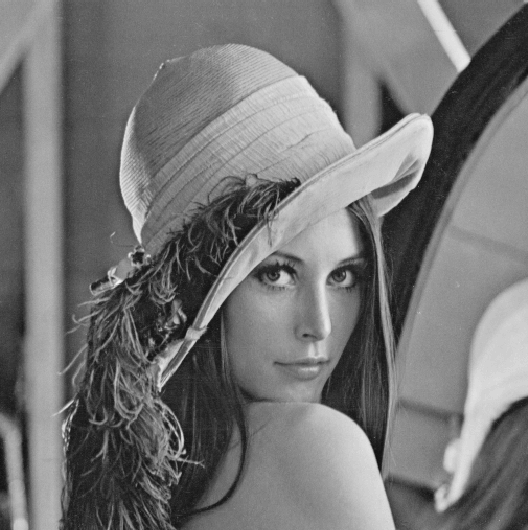
\includegraphics[width=0.24\textwidth]{images/lenaA.png}} 
	\subfigure{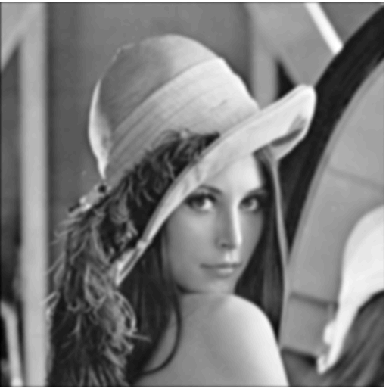
\includegraphics[width=0.24\textwidth]{images/lenaB.png}} 
	\subfigure{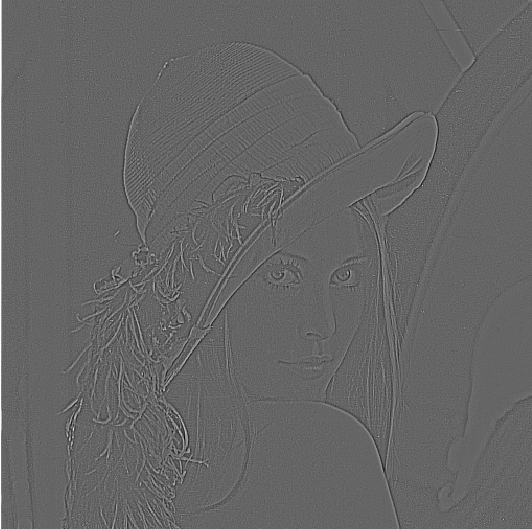
\includegraphics[width=0.24\textwidth]{images/lenaC.png}}
	\subfigure{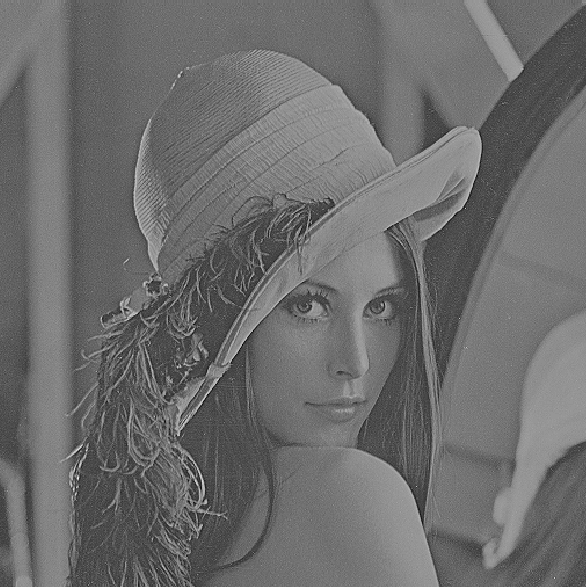
\includegraphics[width=0.24\textwidth]{images/lenaD.png}}
	\caption{Przetworzenie oryginalnego obrazu (najbardziej po lewej stronie) za pomocą operacji splotu z~użyciem różnych filtrów (kolejno rozmycie, wykrywanie krawędzi, wyostrzanie).}
	\label{lab1/fig/imageFiltering}
\end{figure}

W~programie MATLAV/Octave do obliczenia splotu wykorzystuje się funkcję \texttt{conv}, która przyjmuje dwa argumenty będące wektorami dwóch splatanych sygnałów. Obliczenie splotu dwóch wektorów $A$ oraz $B$:
\begin{equation*}
	A=
	\begin{bmatrix}
		1 & 1 & 1
	\end{bmatrix}
\end{equation*}
\begin{equation*}
	B=
	\begin{bmatrix}
		1 & 2 & 3
	\end{bmatrix}
\end{equation*}
w~programie MATLAB/Octave zostało pokazane na poniższym listingu.
\begin{lstlisting}[caption=Obliczanie splotu dwóch wektorów , label=lab1/lst/convolution]
A = [1 1 1];
B = [1 2 3];
C = conv(A,B);
\end{lstlisting}

\begin{figure}[hbt!]
	\centering
	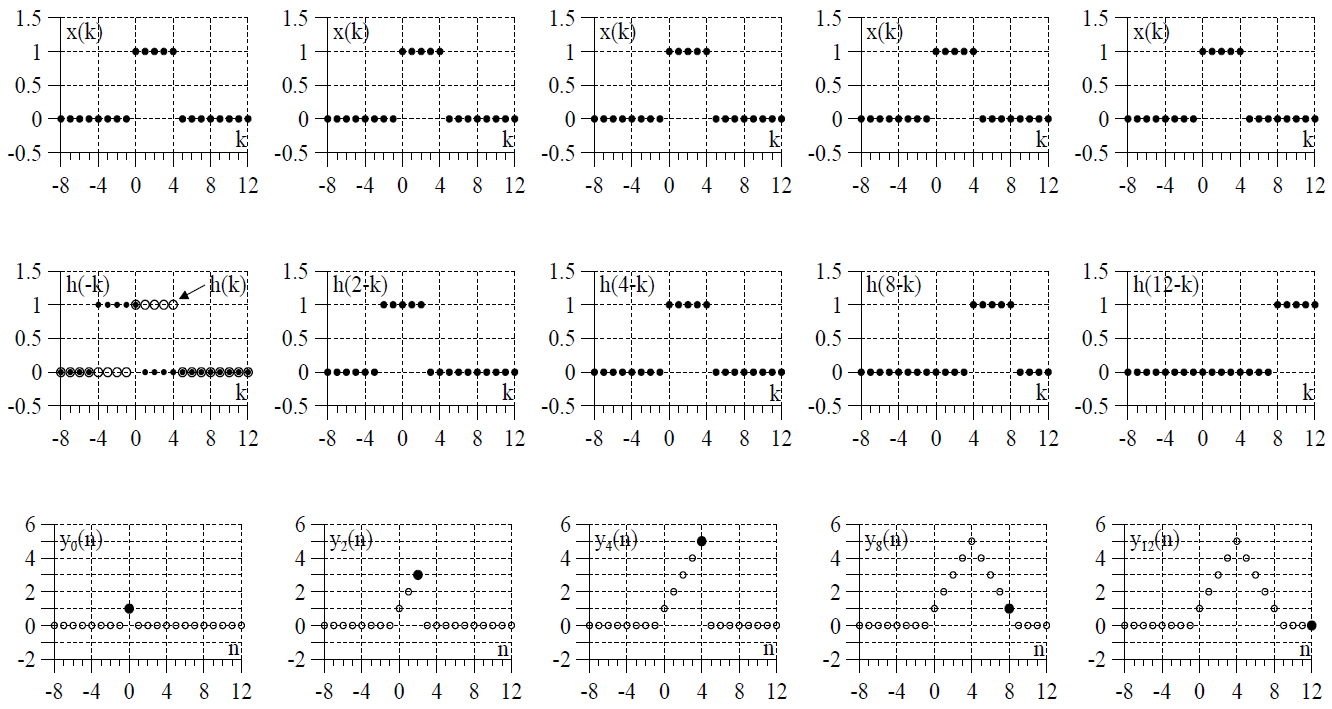
\includegraphics[width=0.9\linewidth]{images/convolution}
	\caption{Graficzna prezentacja splotu dwóch sygnałów prostokątnych~\cite{zielinski_cyfrowe_przetwarzanie_sygnalow}.}
	\label{lab1/fig/convolution}
\end{figure}


\subsection{Zadania}
\subsubsection{Tworznie macierzy}
Korzystając z operatora \texttt{:} stwórz macierz $A$:
\begin{equation*}
	A=
	\begin{bmatrix}
		1 & 1.5 & 2 & 2.5 & 3 & 3.5 & 4 & 4.5 & 5 \\
		-5 & -7 & -9 & -11 & -13 & -15 & -17 & -19 & -21\\
		2 & 4 & 8 & 16 & 32 & 64 & 128 & 256 & 512
	\end{bmatrix}
\end{equation*}
Następnie za pomocą \texttt{[]} usuń drugą, czwartą oraz piątą kolumnę ze stworzonej macierzy. Na koniec dodaj do macierzy $A$ wiersz zawierający same jedynki.

\subsubsection{Rysowanie przebiegów funkcji}
Narysuj na współdzielonym rysunku następujące wykresy (\texttt{subplot}):
\begin{enumerate}
	\item $y(t) = 2sin(2t - \frac{\pi}{2})$,
	\item $y(t) = \frac{10}{t-5} + 20$ (konieczne będzie wykorzystanie operatora dzielenia z~poprzedzającą go kropką (\texttt{./}), pozwoli to na wykonanie dzielenia dla każdego elementu wektora z~osobna),
	\item szum biały o rozkładzie normalnym (stwórz wektor dowolnej długości za pomocą funkcji \texttt{randn}),
	\item przebieg piło-kształtny (wykorzystaj funkcję \texttt{sawtooth}),
	\item przebieg prostokątny (wykorzystaj funkcję \texttt{square}).
\end{enumerate}

\subsubsection{Histogramy wektorów liczb pseudolosowych}
Na podstawie informacji zawartych w rozdziale~\ref{lab1/sec/noises} stwórz dwa wektory zawierające po $10000$ liczb pseudolosowych za pomocą funkcji \texttt{rand} oraz \texttt{randn}. Na współdzielonym wykresie narysuj histogramy (funkcja \texttt{hist}) tych wektorów. Jako pierwszy argument funkcji \texttt{hist} podaj wektor liczb pseudolosowych, jako drugi liczbę słupków histogramu (np. 100) i jako trzeci argument, wartość normalizacyjną (powinna ona wynosić tyle, aby pole pod powierzchnią histogramu wynosiło jeden). Dzięki zastosowaniu normalizacji, histogramy kształtem będą odpowiadać rozkładom gęstości prawdopodobieństwa (rysunek~\ref{lab1/fig/whiteNoisesPdf}). 

 
Korzystając ze wzoru~\ref{lab1/eq/normalDistribution} wyznacz wartości funkcji gęstości prawdopodobieństwa rozkładu normalnego i~nanieś go na drugi ze stworzonych przed chwilą histogramów. Powinny one się pokryć. 

\subsubsection{Filtr średniej ruchomej}
Filtr średniej ruchomej jest specjalnym przypadkiem filtrów o skończonej odpowiedzi impulsowej, którym poświęcimy jedne z~przyszłych laboratoriów. Na ten moment należy jedynie wspomnieć, że filtr średniej ruchomej dodaje do siebie wszystkie wartości filtrowanego sygnału (mieszczące się w oknie tego filtra) i~następnie dzieli je przez długość okna tego filtra~\ref{lab1/eq/movingAverage}.

\begin{equation}\label{lab1/eq/movingAverage}
movAvg = \frac{x[n] + x[n-1] + ... + x[n-N]}{N+1}
\end{equation}

Stwórz sygnał o przebiegu prostokątnym w~tym celu możesz wykorzystać funkcję \texttt{square} (w programie GNU Octave może okazać się konieczne wcześniejsze załadowanie pakietu \texttt{signal}, aby to zrobić wpisz w~wierszu poleceń \texttt{pkg load signal}). Dodaj do tej funkcji biały szum gaussowski (o rozkładzie gaussowskim/normalnych) i~wariancji 0.25 (\texttt{noise = 0.25*rand(size(y,1))}), gdzie \texttt{y} jest wygenerowanym sygnałem prostokątnym.

Utwórz teraz wektor współczynników filtra średniej ruchomej, który ,,spleciony'' z~zaszumionym sygnałem fali prostokątnej pozwoli na zmniejszenie negatywnego wpływu szumu~\ref{lab1/lst/movingAverage}.
\begin{lstlisting}[label=lab1/lst/movingAverage, caption = Przykładowe współczynniki filtra średniej ruchomej]
movAvgLength = 5;
movAvg = 1/movAvgLength * ones(movAvgLength,1);
\end{lstlisting}

Wykorzystaj poznaną funkcję \texttt{conv}, aby obliczyć splot zaszumionego przebiegu z~filtrem średniej ruchomej. Narysuj \textbf{na jednym wykresie} sygnał fali prostokątnej przed i~po filtracji.
 
%\subsubsection{Centralne twierdzenie graniczne}
%W naturze bardzo często możemy się spotkać z~wcześniej omawianym rozkładem normalnym~\ref{lab1/eq/normalDistribution}. Uzasadnieniem powszechności występowania tego rozkładu w przyrodzie, ale również syntetycznych danych jest centralne twierdzenie graniczne. Jeśli dany eksperyment losowy... .Będąc w temacie splotu można powiedzieć, że jeśli \textbf{dowolny} rozkład gęstości prawdopodobieństwa będziemy splatać ze sobą, po kilku takich operacjach będzie coraz bardziej przypominał rozkład normalny.
%
%Utwórz wektor, który będzie odpowiadał dowolnemu rozkładowi gęstości prawdopodobieństwa (nie musisz go normalizować, tak aby całka z~tego rozkładu była równa jeden, tym niemniej pamięta, że pole pod wykresem rozkładu gęstości prawdopodobieństwa zawsze wynosi jeden). Może to być wykres  

%\footnote{
%There's an easier way to create Gaussian randomness at home (or simulated in a computer): take many dice, say 100, throw them all many times, and keep track of the total sum of each throw. If you find the histogram again, you'll see it follows a bell curve. The reason is intuitively easy to grasp: with 100 dice, you're very unlikely to get a total of 100 (all dice would have to land in 1), but it's very easy to get a number around 350, because many different combinations add up to such a number.}



